\documentclass[1p]{elsarticle_modified}
%\bibliographystyle{elsarticle-num}

%\usepackage[colorlinks]{hyperref}
%\usepackage{abbrmath_seonhwa} %\Abb, \Ascr, \Acal ,\Abf, \Afrak
\usepackage{amsfonts}
\usepackage{amssymb}
\usepackage{amsmath}
\usepackage{amsthm}
\usepackage{scalefnt}
\usepackage{amsbsy}
\usepackage{kotex}
\usepackage{caption}
\usepackage{subfig}
\usepackage{color}
\usepackage{graphicx}
\usepackage{xcolor} %% white, black, red, green, blue, cyan, magenta, yellow
\usepackage{float}
\usepackage{setspace}
\usepackage{hyperref}

\usepackage{tikz}
\usetikzlibrary{arrows}

\usepackage{multirow}
\usepackage{array} % fixed length table
\usepackage{hhline}

%%%%%%%%%%%%%%%%%%%%%
\makeatletter
\renewcommand*\env@matrix[1][\arraystretch]{%
	\edef\arraystretch{#1}%
	\hskip -\arraycolsep
	\let\@ifnextchar\new@ifnextchar
	\array{*\c@MaxMatrixCols c}}
\makeatother %https://tex.stackexchange.com/questions/14071/how-can-i-increase-the-line-spacing-in-a-matrix
%%%%%%%%%%%%%%%

\usepackage[normalem]{ulem}

\newcommand{\msout}[1]{\ifmmode\text{\sout{\ensuremath{#1}}}\else\sout{#1}\fi}
%SOURCE: \msout is \stkout macro in https://tex.stackexchange.com/questions/20609/strikeout-in-math-mode

\newcommand{\cancel}[1]{
	\ifmmode
	{\color{red}\msout{#1}}
	\else
	{\color{red}\sout{#1}}
	\fi
}

\newcommand{\add}[1]{
	{\color{blue}\uwave{#1}}
}

\newcommand{\replace}[2]{
	\ifmmode
	{\color{red}\msout{#1}}{\color{blue}\uwave{#2}}
	\else
	{\color{red}\sout{#1}}{\color{blue}\uwave{#2}}
	\fi
}

\newcommand{\Sol}{\mathcal{S}} %segment
\newcommand{\D}{D} %diagram
\newcommand{\A}{\mathcal{A}} %arc


%%%%%%%%%%%%%%%%%%%%%%%%%%%%%5 test

\def\sl{\operatorname{\textup{SL}}(2,\Cbb)}
\def\psl{\operatorname{\textup{PSL}}(2,\Cbb)}
\def\quan{\mkern 1mu \triangleright \mkern 1mu}

\theoremstyle{definition}
\newtheorem{thm}{Theorem}[section]
\newtheorem{prop}[thm]{Proposition}
\newtheorem{lem}[thm]{Lemma}
\newtheorem{ques}[thm]{Question}
\newtheorem{cor}[thm]{Corollary}
\newtheorem{defn}[thm]{Definition}
\newtheorem{exam}[thm]{Example}
\newtheorem{rmk}[thm]{Remark}
\newtheorem{alg}[thm]{Algorithm}

\newcommand{\I}{\sqrt{-1}}
\begin{document}

%\begin{frontmatter}
%
%\title{Boundary parabolic representations of knots up to 8 crossings}
%
%%% Group authors per affiliation:
%\author{Yunhi Cho} 
%\address{Department of Mathematics, University of Seoul, Seoul, Korea}
%\ead{yhcho@uos.ac.kr}
%
%
%\author{Seonhwa Kim} %\fnref{s_kim}}
%\address{Center for Geometry and Physics, Institute for Basic Science, Pohang, 37673, Korea}
%\ead{ryeona17@ibs.re.kr}
%
%\author{Hyuk Kim}
%\address{Department of Mathematical Sciences, Seoul National University, Seoul 08826, Korea}
%\ead{hyukkim@snu.ac.kr}
%
%\author{Seokbeom Yoon}
%\address{Department of Mathematical Sciences, Seoul National University, Seoul, 08826,  Korea}
%\ead{sbyoon15@snu.ac.kr}
%
%\begin{abstract}
%We find all boundary parabolic representation of knots up to 8 crossings.
%
%\end{abstract}
%\begin{keyword}
%    \MSC[2010] 57M25 
%\end{keyword}
%
%\end{frontmatter}

%\linenumbers
%\tableofcontents
%
\newcommand\colored[1]{\textcolor{white}{\rule[-0.35ex]{0.8em}{1.4ex}}\kern-0.8em\color{red} #1}%
%\newcommand\colored[1]{\textcolor{white}{ #1}\kern-2.17ex	\textcolor{white}{ #1}\kern-1.81ex	\textcolor{white}{ #1}\kern-2.15ex\color{red}#1	}

{\Large $\underline{12n_{0287}~(K12n_{0287})}$}

\setlength{\tabcolsep}{10pt}
\renewcommand{\arraystretch}{1.6}
\vspace{1cm}\begin{tabular}{m{100pt}>{\centering\arraybackslash}m{274pt}}
\multirow{5}{120pt}{
	\centering
	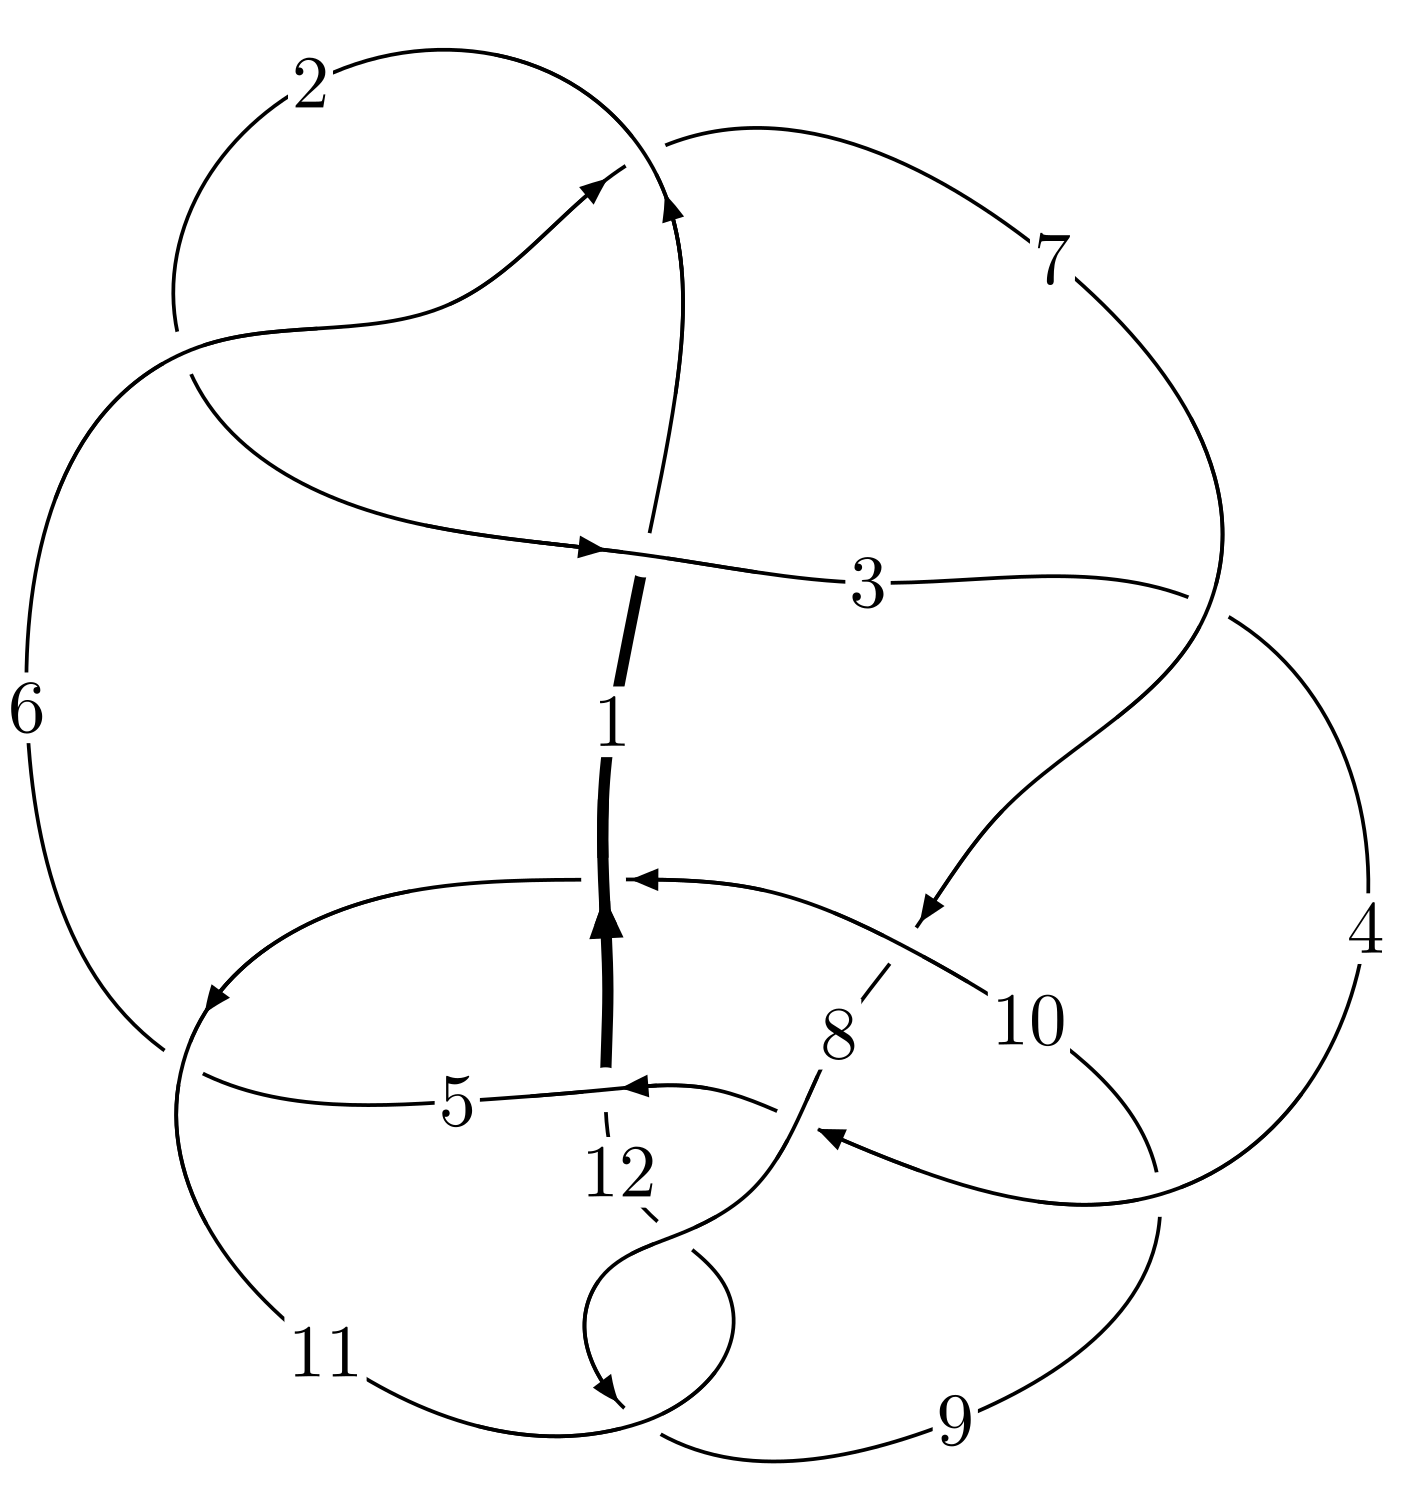
\includegraphics[width=112pt]{../../../GIT/diagram.site/Diagrams/png/2376_12n_0287.png}\\
\ \ \ A knot diagram\footnotemark}&
\allowdisplaybreaks
\textbf{Linearized knot diagam} \\
\cline{2-2}
 &
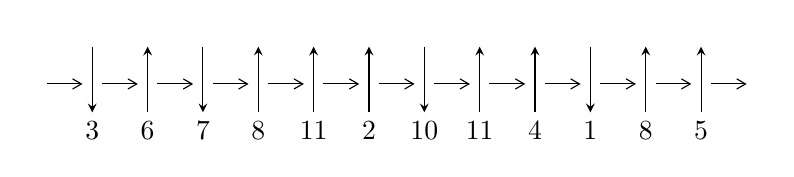
\begin{tikzpicture}[x=20pt, y=17pt]
	% nodes
	\node (C0) at (0, 0) {};
	\node (C1) at (1, 0) {};
	\node (C1U) at (1, +1) {};
	\node (C1D) at (1, -1) {3};

	\node (C2) at (2, 0) {};
	\node (C2U) at (2, +1) {};
	\node (C2D) at (2, -1) {6};

	\node (C3) at (3, 0) {};
	\node (C3U) at (3, +1) {};
	\node (C3D) at (3, -1) {7};

	\node (C4) at (4, 0) {};
	\node (C4U) at (4, +1) {};
	\node (C4D) at (4, -1) {8};

	\node (C5) at (5, 0) {};
	\node (C5U) at (5, +1) {};
	\node (C5D) at (5, -1) {11};

	\node (C6) at (6, 0) {};
	\node (C6U) at (6, +1) {};
	\node (C6D) at (6, -1) {2};

	\node (C7) at (7, 0) {};
	\node (C7U) at (7, +1) {};
	\node (C7D) at (7, -1) {10};

	\node (C8) at (8, 0) {};
	\node (C8U) at (8, +1) {};
	\node (C8D) at (8, -1) {11};

	\node (C9) at (9, 0) {};
	\node (C9U) at (9, +1) {};
	\node (C9D) at (9, -1) {4};

	\node (C10) at (10, 0) {};
	\node (C10U) at (10, +1) {};
	\node (C10D) at (10, -1) {1};

	\node (C11) at (11, 0) {};
	\node (C11U) at (11, +1) {};
	\node (C11D) at (11, -1) {8};

	\node (C12) at (12, 0) {};
	\node (C12U) at (12, +1) {};
	\node (C12D) at (12, -1) {5};
	\node (C13) at (13, 0) {};

	% arrows
	\draw[->,>={angle 60}]
	(C0) edge (C1) (C1) edge (C2) (C2) edge (C3) (C3) edge (C4) (C4) edge (C5) (C5) edge (C6) (C6) edge (C7) (C7) edge (C8) (C8) edge (C9) (C9) edge (C10) (C10) edge (C11) (C11) edge (C12) (C12) edge (C13) ;	\draw[->,>=stealth]
	(C1U) edge (C1D) (C2D) edge (C2U) (C3U) edge (C3D) (C4D) edge (C4U) (C5D) edge (C5U) (C6D) edge (C6U) (C7U) edge (C7D) (C8D) edge (C8U) (C9D) edge (C9U) (C10U) edge (C10D) (C11D) edge (C11U) (C12D) edge (C12U) ;
	\end{tikzpicture} \\
\hhline{~~} \\& 
\textbf{Solving Sequence} \\ \cline{2-2} 
 &
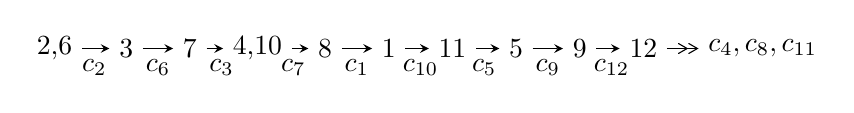
\begin{tikzpicture}[x=23pt, y=7pt]
	% node
	\node (A0) at (-1/8, 0) {2,6};
	\node (A1) at (1, 0) {3};
	\node (A2) at (2, 0) {7};
	\node (A3) at (49/16, 0) {4,10};
	\node (A4) at (33/8, 0) {8};
	\node (A5) at (41/8, 0) {1};
	\node (A6) at (49/8, 0) {11};
	\node (A7) at (57/8, 0) {5};
	\node (A8) at (65/8, 0) {9};
	\node (A9) at (73/8, 0) {12};
	\node (C1) at (1/2, -1) {$c_{2}$};
	\node (C2) at (3/2, -1) {$c_{6}$};
	\node (C3) at (5/2, -1) {$c_{3}$};
	\node (C4) at (29/8, -1) {$c_{7}$};
	\node (C5) at (37/8, -1) {$c_{1}$};
	\node (C6) at (45/8, -1) {$c_{10}$};
	\node (C7) at (53/8, -1) {$c_{5}$};
	\node (C8) at (61/8, -1) {$c_{9}$};
	\node (C9) at (69/8, -1) {$c_{12}$};
	\node (A10) at (11, 0) {$c_{4},c_{8},c_{11}$};

	% edge
	\draw[->,>=stealth]	
	(A0) edge (A1) (A1) edge (A2) (A2) edge (A3) (A3) edge (A4) (A4) edge (A5) (A5) edge (A6) (A6) edge (A7) (A7) edge (A8) (A8) edge (A9) ;
	\draw[->>,>={angle 60}]	
	(A9) edge (A10);
\end{tikzpicture} \\ 

\end{tabular} \\

\footnotetext{
The image of knot diagram is generated by the software ``\textbf{Draw programme}" developed by Andrew Bartholomew(\url{http://www.layer8.co.uk/maths/draw/index.htm\#Running-draw}), where we modified some parts for our purpose(\url{https://github.com/CATsTAILs/LinksPainter}).
}\phantom \\ \newline 
\centering \textbf{Ideals for irreducible components\footnotemark of $X_{\text{par}}$} 
 
\begin{align*}
I^u_{1}&=\langle 
-14 u^{35}-85 u^{34}+\cdots+b-25,\;-27 u^{35}-160 u^{34}+\cdots+2 a-59,\;u^{36}+6 u^{35}+\cdots+11 u+2\rangle \\
I^u_{2}&=\langle 
2 u^{15}+7 u^{13}- u^{12}+12 u^{11}-4 u^{10}+7 u^9-5 u^8-2 u^7- u^6-5 u^5+5 u^4+3 u^2+b- u,\\
\phantom{I^u_{2}}&\phantom{= \langle  }u^{16}+5 u^{14}- u^{13}+11 u^{12}-5 u^{11}+12 u^{10}-10 u^9+4 u^8-8 u^7-3 u^6+2 u^5-3 u^4+8 u^3- u^2+a+3 u-2,\\
\phantom{I^u_{2}}&\phantom{= \langle  }u^{17}- u^{16}+5 u^{15}-4 u^{14}+12 u^{13}-9 u^{12}+16 u^{11}-10 u^{10}+10 u^9-5 u^8+3 u^6-6 u^5+6 u^4-4 u^3+4 u^2-2 u+1\rangle \\
I^u_{3}&=\langle 
- u^{17}+u^{16}+\cdots+b+1,\;u^{17} a+4 u^{17}+\cdots+a^2-5,\;u^{18}- u^{17}+\cdots- u+1\rangle \\
\\
\end{align*}
\raggedright * 3 irreducible components of $\dim_{\mathbb{C}}=0$, with total 89 representations.\\
\footnotetext{All coefficients of polynomials are rational numbers. But the coefficients are sometimes approximated in decimal forms when there is not enough margin.}
\newpage
\renewcommand{\arraystretch}{1}
\centering \section*{I. $I^u_{1}= \langle -14 u^{35}-85 u^{34}+\cdots+b-25,\;-27 u^{35}-160 u^{34}+\cdots+2 a-59,\;u^{36}+6 u^{35}+\cdots+11 u+2 \rangle$}
\flushleft \textbf{(i) Arc colorings}\\
\begin{tabular}{m{7pt} m{180pt} m{7pt} m{180pt} }
\flushright $a_{2}=$&$\begin{pmatrix}1\\0\end{pmatrix}$ \\
\flushright $a_{6}=$&$\begin{pmatrix}0\\u\end{pmatrix}$ \\
\flushright $a_{3}=$&$\begin{pmatrix}1\\- u^2\end{pmatrix}$ \\
\flushright $a_{7}=$&$\begin{pmatrix}u\\u\end{pmatrix}$ \\
\flushright $a_{4}=$&$\begin{pmatrix}u^4+u^2+1\\u^4\end{pmatrix}$ \\
\flushright $a_{10}=$&$\begin{pmatrix}\frac{27}{2} u^{35}+80 u^{34}+\cdots+\frac{287}{2} u+\frac{59}{2}\\14 u^{35}+85 u^{34}+\cdots+135 u+25\end{pmatrix}$ \\
\flushright $a_{8}=$&$\begin{pmatrix}\frac{5}{2} u^{35}+15 u^{34}+\cdots+\frac{55}{2} u+\frac{13}{2}\\3 u^{35}+17 u^{34}+\cdots+27 u+5\end{pmatrix}$ \\
\flushright $a_{1}=$&$\begin{pmatrix}u^2+1\\- u^4\end{pmatrix}$ \\
\flushright $a_{11}=$&$\begin{pmatrix}\frac{17}{2} u^{35}+51 u^{34}+\cdots+\frac{205}{2} u+\frac{41}{2}\\5 u^{35}+36 u^{34}+\cdots+85 u+17\end{pmatrix}$ \\
\flushright $a_{5}=$&$\begin{pmatrix}-\frac{1}{2} u^{35}-5 u^{34}+\cdots+\frac{1}{2} u+\frac{3}{2}\\-2 u^{35}-14 u^{34}+\cdots-19 u-3\end{pmatrix}$ \\
\flushright $a_{9}=$&$\begin{pmatrix}\frac{7}{2} u^{35}+21 u^{34}+\cdots+\frac{85}{2} u+\frac{17}{2}\\u^{35}+6 u^{34}+\cdots+30 u+7\end{pmatrix}$ \\
\flushright $a_{12}=$&$\begin{pmatrix}\frac{13}{2} u^{35}+38 u^{34}+\cdots+\frac{121}{2} u+\frac{27}{2}\\11 u^{35}+63 u^{34}+\cdots+69 u+11\end{pmatrix}$\\&\end{tabular}
\flushleft \textbf{(ii) Obstruction class $= -1$}\\~\\
\flushleft \textbf{(iii) Cusp Shapes $= -10 u^{35}-47 u^{34}-193 u^{33}-528 u^{32}-1308 u^{31}-2680 u^{30}-5100 u^{29}-8677 u^{28}-13841 u^{27}-20439 u^{26}-28425 u^{25}-37282 u^{24}-46259 u^{23}-54570 u^{22}-61115 u^{21}-65180 u^{20}-66272 u^{19}-64122 u^{18}-59268 u^{17}-52003 u^{16}-43524 u^{15}-34581 u^{14}-26106 u^{13}-18689 u^{12}-12638 u^{11}-8103 u^{10}-4980 u^9-2882 u^8-1585 u^7-744 u^6-322 u^5-123 u^4-56 u^3-11 u^2+11 u+16$}\\~\\
\newpage\renewcommand{\arraystretch}{1}
\flushleft \textbf{(iv) u-Polynomials at the component}\newline \\
\begin{tabular}{m{50pt}|m{274pt}}
Crossings & \hspace{64pt}u-Polynomials at each crossing \\
\hline $$\begin{aligned}c_{1}\end{aligned}$$&$\begin{aligned}
&u^{36}+18 u^{35}+\cdots+11 u+4
\end{aligned}$\\
\hline $$\begin{aligned}c_{2},c_{6}\end{aligned}$$&$\begin{aligned}
&u^{36}-6 u^{35}+\cdots-11 u+2
\end{aligned}$\\
\hline $$\begin{aligned}c_{3}\end{aligned}$$&$\begin{aligned}
&u^{36}+6 u^{35}+\cdots+721 u+74
\end{aligned}$\\
\hline $$\begin{aligned}c_{4},c_{12}\end{aligned}$$&$\begin{aligned}
&u^{36}-28 u^{34}+\cdots+u+1
\end{aligned}$\\
\hline $$\begin{aligned}c_{5},c_{9}\end{aligned}$$&$\begin{aligned}
&u^{36}-8 u^{34}+\cdots-19 u+23
\end{aligned}$\\
\hline $$\begin{aligned}c_{7},c_{10}\end{aligned}$$&$\begin{aligned}
&u^{36}-3 u^{35}+\cdots-4 u+1
\end{aligned}$\\
\hline $$\begin{aligned}c_{8},c_{11}\end{aligned}$$&$\begin{aligned}
&u^{36}+17 u^{35}+\cdots-1495 u+160
\end{aligned}$\\
\hline
\end{tabular}\\~\\
\newpage\renewcommand{\arraystretch}{1}
\flushleft \textbf{(v) Riley Polynomials at the component}\newline \\
\begin{tabular}{m{50pt}|m{274pt}}
Crossings & \hspace{64pt}Riley Polynomials at each crossing \\
\hline $$\begin{aligned}c_{1}\end{aligned}$$&$\begin{aligned}
&y^{36}+2 y^{35}+\cdots+415 y+16
\end{aligned}$\\
\hline $$\begin{aligned}c_{2},c_{6}\end{aligned}$$&$\begin{aligned}
&y^{36}+18 y^{35}+\cdots+11 y+4
\end{aligned}$\\
\hline $$\begin{aligned}c_{3}\end{aligned}$$&$\begin{aligned}
&y^{36}-20 y^{35}+\cdots-111805 y+5476
\end{aligned}$\\
\hline $$\begin{aligned}c_{4},c_{12}\end{aligned}$$&$\begin{aligned}
&y^{36}-56 y^{35}+\cdots- y+1
\end{aligned}$\\
\hline $$\begin{aligned}c_{5},c_{9}\end{aligned}$$&$\begin{aligned}
&y^{36}-16 y^{35}+\cdots-5421 y+529
\end{aligned}$\\
\hline $$\begin{aligned}c_{7},c_{10}\end{aligned}$$&$\begin{aligned}
&y^{36}+9 y^{35}+\cdots+16 y+1
\end{aligned}$\\
\hline $$\begin{aligned}c_{8},c_{11}\end{aligned}$$&$\begin{aligned}
&y^{36}-29 y^{35}+\cdots-1047185 y+25600
\end{aligned}$\\
\hline
\end{tabular}\\~\\
\newpage\flushleft \textbf{(vi) Complex Volumes and Cusp Shapes}
$$\begin{array}{c|c|c}  
\text{Solutions to }I^u_{1}& \I (\text{vol} + \sqrt{-1}CS) & \text{Cusp shape}\\
 \hline 
\begin{aligned}
u &= -0.149973 + 0.998728 I \\
a &= \phantom{-}0.826426 + 0.069933 I \\
b &= \phantom{-}0.978572 - 0.499137 I\end{aligned}
 & -2.48443 - 1.62652 I & -2.33035 + 4.22312 I \\ \hline\begin{aligned}
u &= -0.149973 - 0.998728 I \\
a &= \phantom{-}0.826426 - 0.069933 I \\
b &= \phantom{-}0.978572 + 0.499137 I\end{aligned}
 & -2.48443 + 1.62652 I & -2.33035 - 4.22312 I \\ \hline\begin{aligned}
u &= -0.991952 + 0.201272 I \\
a &= -0.095835 - 0.534611 I \\
b &= \phantom{-}0.1012230 - 0.0449035 I\end{aligned}
 & \phantom{-}5.44078 - 0.44653 I & \phantom{-}17.6525 + 14.6221 I \\ \hline\begin{aligned}
u &= -0.991952 - 0.201272 I \\
a &= -0.095835 + 0.534611 I \\
b &= \phantom{-}0.1012230 + 0.0449035 I\end{aligned}
 & \phantom{-}5.44078 + 0.44653 I & \phantom{-}17.6525 - 14.6221 I \\ \hline\begin{aligned}
u &= \phantom{-}0.722213 + 0.749533 I \\
a &= -0.458236 - 0.270213 I \\
b &= -0.182561 + 1.023860 I\end{aligned}
 & \phantom{-}10.02280 + 8.45449 I & \phantom{-}8.41836 - 6.51159 I \\ \hline\begin{aligned}
u &= \phantom{-}0.722213 - 0.749533 I \\
a &= -0.458236 + 0.270213 I \\
b &= -0.182561 - 1.023860 I\end{aligned}
 & \phantom{-}10.02280 - 8.45449 I & \phantom{-}8.41836 + 6.51159 I \\ \hline\begin{aligned}
u &= \phantom{-}0.704411 + 0.851124 I \\
a &= \phantom{-}0.304244 - 0.316418 I \\
b &= -0.793602 - 0.473087 I\end{aligned}
 & \phantom{-}9.73048 - 3.08341 I & \phantom{-}8.49473 + 1.45967 I \\ \hline\begin{aligned}
u &= \phantom{-}0.704411 - 0.851124 I \\
a &= \phantom{-}0.304244 + 0.316418 I \\
b &= -0.793602 + 0.473087 I\end{aligned}
 & \phantom{-}9.73048 + 3.08341 I & \phantom{-}8.49473 - 1.45967 I \\ \hline\begin{aligned}
u &= -0.839708 + 0.298444 I \\
a &= -2.16620 + 0.59359 I \\
b &= -0.604870 - 0.306470 I\end{aligned}
 & \phantom{-}7.48792 + 11.15390 I & \phantom{-}7.02947 - 5.33510 I \\ \hline\begin{aligned}
u &= -0.839708 - 0.298444 I \\
a &= -2.16620 - 0.59359 I \\
b &= -0.604870 + 0.306470 I\end{aligned}
 & \phantom{-}7.48792 - 11.15390 I & \phantom{-}7.02947 + 5.33510 I\\
 \hline 
 \end{array}$$\newpage$$\begin{array}{c|c|c}  
\text{Solutions to }I^u_{1}& \I (\text{vol} + \sqrt{-1}CS) & \text{Cusp shape}\\
 \hline 
\begin{aligned}
u &= \phantom{-}0.459586 + 1.035300 I \\
a &= -0.189766 + 0.533405 I \\
b &= \phantom{-}0.983727 + 0.590961 I\end{aligned}
 & -0.955654 + 0.821545 I & \phantom{-0.000000 } 0. - 3.95614 I \\ \hline\begin{aligned}
u &= \phantom{-}0.459586 - 1.035300 I \\
a &= -0.189766 - 0.533405 I \\
b &= \phantom{-}0.983727 - 0.590961 I\end{aligned}
 & -0.955654 - 0.821545 I & \phantom{-0.000000 -}0. + 3.95614 I \\ \hline\begin{aligned}
u &= -0.349884 + 1.107310 I \\
a &= -0.40589 - 1.81289 I \\
b &= -1.19270 - 2.50026 I\end{aligned}
 & -4.05377 + 0.63572 I & \phantom{-}0.484295 - 0.443572 I \\ \hline\begin{aligned}
u &= -0.349884 - 1.107310 I \\
a &= -0.40589 + 1.81289 I \\
b &= -1.19270 + 2.50026 I\end{aligned}
 & -4.05377 - 0.63572 I & \phantom{-}0.484295 + 0.443572 I \\ \hline\begin{aligned}
u &= \phantom{-}0.489524 + 1.057530 I \\
a &= \phantom{-}0.323550 - 0.327963 I \\
b &= -0.560466 - 0.804802 I\end{aligned}
 & -0.66063 + 5.65062 I & \phantom{-}0.65729 - 7.68260 I \\ \hline\begin{aligned}
u &= \phantom{-}0.489524 - 1.057530 I \\
a &= \phantom{-}0.323550 + 0.327963 I \\
b &= -0.560466 + 0.804802 I\end{aligned}
 & -0.66063 - 5.65062 I & \phantom{-}0.65729 + 7.68260 I \\ \hline\begin{aligned}
u &= -0.477205 + 1.078410 I \\
a &= -0.219824 + 1.300630 I \\
b &= -0.24654 + 1.84787 I\end{aligned}
 & -0.93062 - 3.45682 I & \phantom{-}3.69827 + 2.78118 I \\ \hline\begin{aligned}
u &= -0.477205 - 1.078410 I \\
a &= -0.219824 - 1.300630 I \\
b &= -0.24654 - 1.84787 I\end{aligned}
 & -0.93062 + 3.45682 I & \phantom{-}3.69827 - 2.78118 I \\ \hline\begin{aligned}
u &= -0.516662 + 1.118490 I \\
a &= \phantom{-}0.37409 - 2.28317 I \\
b &= \phantom{-}0.64651 - 3.41250 I\end{aligned}
 & -2.89301 - 8.21064 I & \phantom{-}2.73606 + 6.67381 I \\ \hline\begin{aligned}
u &= -0.516662 - 1.118490 I \\
a &= \phantom{-}0.37409 + 2.28317 I \\
b &= \phantom{-}0.64651 + 3.41250 I\end{aligned}
 & -2.89301 + 8.21064 I & \phantom{-}2.73606 - 6.67381 I\\
 \hline 
 \end{array}$$\newpage$$\begin{array}{c|c|c}  
\text{Solutions to }I^u_{1}& \I (\text{vol} + \sqrt{-1}CS) & \text{Cusp shape}\\
 \hline 
\begin{aligned}
u &= -0.235187 + 1.215000 I \\
a &= \phantom{-}0.269343 + 1.318210 I \\
b &= \phantom{-}1.29431 + 2.00975 I\end{aligned}
 & \phantom{-}2.56736 + 7.86975 I & \phantom{-}1.57367 - 3.75977 I \\ \hline\begin{aligned}
u &= -0.235187 - 1.215000 I \\
a &= \phantom{-}0.269343 - 1.318210 I \\
b &= \phantom{-}1.29431 - 2.00975 I\end{aligned}
 & \phantom{-}2.56736 - 7.86975 I & \phantom{-}1.57367 + 3.75977 I \\ \hline\begin{aligned}
u &= \phantom{-}0.437735 + 0.549718 I \\
a &= \phantom{-}0.890033 + 0.585768 I \\
b &= \phantom{-}0.312734 - 1.109250 I\end{aligned}
 & \phantom{-}0.56302 + 2.97658 I & \phantom{-}7.22028 + 1.12421 I \\ \hline\begin{aligned}
u &= \phantom{-}0.437735 - 0.549718 I \\
a &= \phantom{-}0.890033 - 0.585768 I \\
b &= \phantom{-}0.312734 + 1.109250 I\end{aligned}
 & \phantom{-}0.56302 - 2.97658 I & \phantom{-}7.22028 - 1.12421 I \\ \hline\begin{aligned}
u &= -0.579068 + 1.162280 I \\
a &= -0.18131 + 2.07088 I \\
b &= -0.66974 + 3.26898 I\end{aligned}
 & \phantom{-}4.9093 - 16.4009 I & \phantom{-}4.03368 + 8.81881 I \\ \hline\begin{aligned}
u &= -0.579068 - 1.162280 I \\
a &= -0.18131 - 2.07088 I \\
b &= -0.66974 - 3.26898 I\end{aligned}
 & \phantom{-}4.9093 + 16.4009 I & \phantom{-}4.03368 - 8.81881 I \\ \hline\begin{aligned}
u &= -0.645401 + 0.250421 I \\
a &= \phantom{-}2.56211 - 0.68246 I \\
b &= \phantom{-}0.796733 - 0.012403 I\end{aligned}
 & -0.44102 + 3.68764 I & \phantom{-}6.93148 - 2.97663 I \\ \hline\begin{aligned}
u &= -0.645401 - 0.250421 I \\
a &= \phantom{-}2.56211 + 0.68246 I \\
b &= \phantom{-}0.796733 + 0.012403 I\end{aligned}
 & -0.44102 - 3.68764 I & \phantom{-}6.93148 + 2.97663 I \\ \hline\begin{aligned}
u &= -0.379298 + 1.270510 I \\
a &= -0.367307 + 0.599503 I \\
b &= -0.495507 + 1.221510 I\end{aligned}
 & \phantom{-}0.75632 - 4.99885 I & \phantom{-0.000000 -}0. + 9.16274 I \\ \hline\begin{aligned}
u &= -0.379298 - 1.270510 I \\
a &= -0.367307 - 0.599503 I \\
b &= -0.495507 - 1.221510 I\end{aligned}
 & \phantom{-}0.75632 + 4.99885 I & \phantom{-0.000000 } 0. - 9.16274 I\\
 \hline 
 \end{array}$$\newpage$$\begin{array}{c|c|c}  
\text{Solutions to }I^u_{1}& \I (\text{vol} + \sqrt{-1}CS) & \text{Cusp shape}\\
 \hline 
\begin{aligned}
u &= \phantom{-}0.507489 + 0.424879 I \\
a &= -0.697425 - 0.253280 I \\
b &= \phantom{-}0.190814 + 0.745125 I\end{aligned}
 & \phantom{-}1.18510 - 1.52172 I & \phantom{-}5.49872 + 4.62592 I \\ \hline\begin{aligned}
u &= \phantom{-}0.507489 - 0.424879 I \\
a &= -0.697425 + 0.253280 I \\
b &= \phantom{-}0.190814 - 0.745125 I\end{aligned}
 & \phantom{-}1.18510 + 1.52172 I & \phantom{-}5.49872 - 4.62592 I \\ \hline\begin{aligned}
u &= -0.505579 + 0.388688 I \\
a &= -1.192940 + 0.572586 I \\
b &= -0.480909 + 0.224460 I\end{aligned}
 & \phantom{-}1.086520 - 0.606535 I & \phantom{-}7.97928 + 3.45064 I \\ \hline\begin{aligned}
u &= -0.505579 - 0.388688 I \\
a &= -1.192940 - 0.572586 I \\
b &= -0.480909 - 0.224460 I\end{aligned}
 & \phantom{-}1.086520 + 0.606535 I & \phantom{-}7.97928 - 3.45064 I \\ \hline\begin{aligned}
u &= -0.651042 + 1.222950 I \\
a &= \phantom{-}0.174939 - 0.327220 I \\
b &= \phantom{-}0.422269 - 0.499103 I\end{aligned}
 & \phantom{-}2.39061 - 5.47394 I & \phantom{-}20.9532 + 20.3381 I \\ \hline\begin{aligned}
u &= -0.651042 - 1.222950 I \\
a &= \phantom{-}0.174939 + 0.327220 I \\
b &= \phantom{-}0.422269 + 0.499103 I\end{aligned}
 & \phantom{-}2.39061 + 5.47394 I & \phantom{-}20.9532 - 20.3381 I\\
 \hline 
 \end{array}$$\newpage\newpage\renewcommand{\arraystretch}{1}
\centering \section*{II. $I^u_{2}= \langle 2 u^{15}+7 u^{13}+\cdots+b- u,\;u^{16}+5 u^{14}+\cdots+a-2,\;u^{17}- u^{16}+\cdots-2 u+1 \rangle$}
\flushleft \textbf{(i) Arc colorings}\\
\begin{tabular}{m{7pt} m{180pt} m{7pt} m{180pt} }
\flushright $a_{2}=$&$\begin{pmatrix}1\\0\end{pmatrix}$ \\
\flushright $a_{6}=$&$\begin{pmatrix}0\\u\end{pmatrix}$ \\
\flushright $a_{3}=$&$\begin{pmatrix}1\\- u^2\end{pmatrix}$ \\
\flushright $a_{7}=$&$\begin{pmatrix}u\\u\end{pmatrix}$ \\
\flushright $a_{4}=$&$\begin{pmatrix}u^4+u^2+1\\u^4\end{pmatrix}$ \\
\flushright $a_{10}=$&$\begin{pmatrix}- u^{16}-5 u^{14}+\cdots-3 u+2\\-2 u^{15}-7 u^{13}+\cdots-3 u^2+u\end{pmatrix}$ \\
\flushright $a_{8}=$&$\begin{pmatrix}2 u^{16}- u^{15}+\cdots+4 u-3\\u^{16}+5 u^{14}+\cdots+2 u-1\end{pmatrix}$ \\
\flushright $a_{1}=$&$\begin{pmatrix}u^2+1\\- u^4\end{pmatrix}$ \\
\flushright $a_{11}=$&$\begin{pmatrix}-2 u^{16}+u^{15}+\cdots-4 u+2\\- u^{16}-4 u^{14}+\cdots- u+1\end{pmatrix}$ \\
\flushright $a_{5}=$&$\begin{pmatrix}3 u^{16}-5 u^{15}+\cdots+11 u-7\\u^{16}-4 u^{15}+\cdots+6 u-5\end{pmatrix}$ \\
\flushright $a_{9}=$&$\begin{pmatrix}-2 u^{16}+u^{15}+\cdots-5 u+2\\- u^{16}+u^{15}+\cdots-2 u+2\end{pmatrix}$ \\
\flushright $a_{12}=$&$\begin{pmatrix}-5 u^{16}+2 u^{15}+\cdots-12 u+8\\-2 u^{16}-2 u^{15}+\cdots-2 u+2\end{pmatrix}$\\&\end{tabular}
\flushleft \textbf{(ii) Obstruction class $= 1$}\\~\\
\flushleft \textbf{(iii) Cusp Shapes $= 6 u^{15}-4 u^{14}+24 u^{13}-12 u^{12}+48 u^{11}-20 u^{10}+44 u^9-6 u^8+6 u^7+12 u^6-21 u^5+22 u^4-14 u^3+10 u^2- u+6$}\\~\\
\newpage\renewcommand{\arraystretch}{1}
\flushleft \textbf{(iv) u-Polynomials at the component}\newline \\
\begin{tabular}{m{50pt}|m{274pt}}
Crossings & \hspace{64pt}u-Polynomials at each crossing \\
\hline $$\begin{aligned}c_{1}\end{aligned}$$&$\begin{aligned}
&u^{17}-9 u^{16}+\cdots-4 u+1
\end{aligned}$\\
\hline $$\begin{aligned}c_{2}\end{aligned}$$&$\begin{aligned}
&u^{17}- u^{16}+\cdots-2 u+1
\end{aligned}$\\
\hline $$\begin{aligned}c_{3}\end{aligned}$$&$\begin{aligned}
&u^{17}+u^{16}+\cdots+2 u+5
\end{aligned}$\\
\hline $$\begin{aligned}c_{4},c_{12}\end{aligned}$$&$\begin{aligned}
&u^{17}-2 u^{16}+\cdots-3 u+1
\end{aligned}$\\
\hline $$\begin{aligned}c_{5},c_{9}\end{aligned}$$&$\begin{aligned}
&u^{17}-8 u^{15}+\cdots- u+1
\end{aligned}$\\
\hline $$\begin{aligned}c_{6}\end{aligned}$$&$\begin{aligned}
&u^{17}+u^{16}+\cdots-2 u-1
\end{aligned}$\\
\hline $$\begin{aligned}c_{7},c_{10}\end{aligned}$$&$\begin{aligned}
&u^{17}-3 u^{16}+\cdots+2 u+1
\end{aligned}$\\
\hline $$\begin{aligned}c_{8}\end{aligned}$$&$\begin{aligned}
&u^{17}+14 u^{16}+\cdots+23 u+5
\end{aligned}$\\
\hline $$\begin{aligned}c_{11}\end{aligned}$$&$\begin{aligned}
&u^{17}-14 u^{16}+\cdots+23 u-5
\end{aligned}$\\
\hline
\end{tabular}\\~\\
\newpage\renewcommand{\arraystretch}{1}
\flushleft \textbf{(v) Riley Polynomials at the component}\newline \\
\begin{tabular}{m{50pt}|m{274pt}}
Crossings & \hspace{64pt}Riley Polynomials at each crossing \\
\hline $$\begin{aligned}c_{1}\end{aligned}$$&$\begin{aligned}
&y^{17}+y^{16}+\cdots-8 y-1
\end{aligned}$\\
\hline $$\begin{aligned}c_{2},c_{6}\end{aligned}$$&$\begin{aligned}
&y^{17}+9 y^{16}+\cdots-4 y-1
\end{aligned}$\\
\hline $$\begin{aligned}c_{3}\end{aligned}$$&$\begin{aligned}
&y^{17}-13 y^{16}+\cdots-86 y-25
\end{aligned}$\\
\hline $$\begin{aligned}c_{4},c_{12}\end{aligned}$$&$\begin{aligned}
&y^{17}-16 y^{16}+\cdots-3 y-1
\end{aligned}$\\
\hline $$\begin{aligned}c_{5},c_{9}\end{aligned}$$&$\begin{aligned}
&y^{17}-16 y^{16}+\cdots+9 y-1
\end{aligned}$\\
\hline $$\begin{aligned}c_{7},c_{10}\end{aligned}$$&$\begin{aligned}
&y^{17}-7 y^{16}+\cdots+4 y-1
\end{aligned}$\\
\hline $$\begin{aligned}c_{8},c_{11}\end{aligned}$$&$\begin{aligned}
&y^{17}-18 y^{16}+\cdots-371 y-25
\end{aligned}$\\
\hline
\end{tabular}\\~\\
\newpage\flushleft \textbf{(vi) Complex Volumes and Cusp Shapes}
$$\begin{array}{c|c|c}  
\text{Solutions to }I^u_{2}& \I (\text{vol} + \sqrt{-1}CS) & \text{Cusp shape}\\
 \hline 
\begin{aligned}
u &= -0.431008 + 0.942233 I \\
a &= \phantom{-}0.209460 + 0.502451 I \\
b &= -0.824758 + 0.503665 I\end{aligned}
 & -0.436145 - 0.105477 I & \phantom{-}5.17968 - 2.38886 I \\ \hline\begin{aligned}
u &= -0.431008 - 0.942233 I \\
a &= \phantom{-}0.209460 - 0.502451 I \\
b &= -0.824758 - 0.503665 I\end{aligned}
 & -0.436145 + 0.105477 I & \phantom{-}5.17968 + 2.38886 I \\ \hline\begin{aligned}
u &= -0.874680\phantom{ +0.000000I} \\
a &= -0.192244\phantom{ +0.000000I} \\
b &= \phantom{-}0.315231\phantom{ +0.000000I}\end{aligned}
 & \phantom{-}5.41472\phantom{ +0.000000I} & \phantom{-}11.0230\phantom{ +0.000000I} \\ \hline\begin{aligned}
u &= -0.468457 + 0.715892 I \\
a &= -0.678237 + 0.210938 I \\
b &= -0.173523 - 0.977457 I\end{aligned}
 & \phantom{-}0.24900 - 3.62004 I & \phantom{-}1.98563 + 8.95063 I \\ \hline\begin{aligned}
u &= -0.468457 - 0.715892 I \\
a &= -0.678237 - 0.210938 I \\
b &= -0.173523 + 0.977457 I\end{aligned}
 & \phantom{-}0.24900 + 3.62004 I & \phantom{-}1.98563 - 8.95063 I \\ \hline\begin{aligned}
u &= \phantom{-}0.464004 + 1.050320 I \\
a &= -0.31217 + 3.03749 I \\
b &= -0.65170 + 4.08273 I\end{aligned}
 & \phantom{-}5.02616 + 3.30361 I & \phantom{-}0.39237 - 4.97703 I \\ \hline\begin{aligned}
u &= \phantom{-}0.464004 - 1.050320 I \\
a &= -0.31217 - 3.03749 I \\
b &= -0.65170 - 4.08273 I\end{aligned}
 & \phantom{-}5.02616 - 3.30361 I & \phantom{-}0.39237 + 4.97703 I \\ \hline\begin{aligned}
u &= \phantom{-}0.773218 + 0.228170 I \\
a &= -1.92418 - 0.33198 I \\
b &= -0.478975 + 0.164410 I\end{aligned}
 & -2.06386 - 4.46334 I & \phantom{-}0.46360 + 4.84315 I \\ \hline\begin{aligned}
u &= \phantom{-}0.773218 - 0.228170 I \\
a &= -1.92418 + 0.33198 I \\
b &= -0.478975 - 0.164410 I\end{aligned}
 & -2.06386 + 4.46334 I & \phantom{-}0.46360 - 4.84315 I \\ \hline\begin{aligned}
u &= \phantom{-}0.305634 + 1.188350 I \\
a &= \phantom{-}0.051305 - 1.236500 I \\
b &= \phantom{-}0.65454 - 1.98487 I\end{aligned}
 & -6.36852 - 1.01335 I & -5.48366 + 1.62767 I\\
 \hline 
 \end{array}$$\newpage$$\begin{array}{c|c|c}  
\text{Solutions to }I^u_{2}& \I (\text{vol} + \sqrt{-1}CS) & \text{Cusp shape}\\
 \hline 
\begin{aligned}
u &= \phantom{-}0.305634 - 1.188350 I \\
a &= \phantom{-}0.051305 + 1.236500 I \\
b &= \phantom{-}0.65454 + 1.98487 I\end{aligned}
 & -6.36852 + 1.01335 I & -5.48366 - 1.62767 I \\ \hline\begin{aligned}
u &= \phantom{-}0.539603 + 1.156090 I \\
a &= -0.00613 - 1.80864 I \\
b &= -0.17533 - 2.86609 I\end{aligned}
 & -4.76857 + 9.35771 I & -2.38330 - 7.93311 I \\ \hline\begin{aligned}
u &= \phantom{-}0.539603 - 1.156090 I \\
a &= -0.00613 + 1.80864 I \\
b &= -0.17533 + 2.86609 I\end{aligned}
 & -4.76857 - 9.35771 I & -2.38330 + 7.93311 I \\ \hline\begin{aligned}
u &= -0.596101 + 1.176370 I \\
a &= -0.0194796 - 0.1364700 I \\
b &= \phantom{-}0.343510 - 0.109245 I\end{aligned}
 & \phantom{-}2.18794 - 5.27328 I & -0.326316 - 0.621275 I \\ \hline\begin{aligned}
u &= -0.596101 - 1.176370 I \\
a &= -0.0194796 + 0.1364700 I \\
b &= \phantom{-}0.343510 + 0.109245 I\end{aligned}
 & \phantom{-}2.18794 + 5.27328 I & -0.326316 + 0.621275 I \\ \hline\begin{aligned}
u &= \phantom{-}0.350446 + 0.524920 I \\
a &= \phantom{-}2.77555 - 1.60523 I \\
b &= \phantom{-}1.64862 - 0.37193 I\end{aligned}
 & \phantom{-}6.75650 + 0.40196 I & \phantom{-}5.16061 + 1.96558 I \\ \hline\begin{aligned}
u &= \phantom{-}0.350446 - 0.524920 I \\
a &= \phantom{-}2.77555 + 1.60523 I \\
b &= \phantom{-}1.64862 + 0.37193 I\end{aligned}
 & \phantom{-}6.75650 - 0.40196 I & \phantom{-}5.16061 - 1.96558 I\\
 \hline 
 \end{array}$$\newpage\newpage\renewcommand{\arraystretch}{1}
\centering \section*{III. $I^u_{3}= \langle - u^{17}+u^{16}+\cdots+b+1,\;u^{17} a+4 u^{17}+\cdots+a^2-5,\;u^{18}- u^{17}+\cdots- u+1 \rangle$}
\flushleft \textbf{(i) Arc colorings}\\
\begin{tabular}{m{7pt} m{180pt} m{7pt} m{180pt} }
\flushright $a_{2}=$&$\begin{pmatrix}1\\0\end{pmatrix}$ \\
\flushright $a_{6}=$&$\begin{pmatrix}0\\u\end{pmatrix}$ \\
\flushright $a_{3}=$&$\begin{pmatrix}1\\- u^2\end{pmatrix}$ \\
\flushright $a_{7}=$&$\begin{pmatrix}u\\u\end{pmatrix}$ \\
\flushright $a_{4}=$&$\begin{pmatrix}u^4+u^2+1\\u^4\end{pmatrix}$ \\
\flushright $a_{10}=$&$\begin{pmatrix}a\\u^{17}- u^{16}+\cdots+u-1\end{pmatrix}$ \\
\flushright $a_{8}=$&$\begin{pmatrix}- u^{17}+u^{16}+\cdots- a-1\\-2 u^{17}+2 u^{16}+\cdots-2 u+1\end{pmatrix}$ \\
\flushright $a_{1}=$&$\begin{pmatrix}u^2+1\\- u^4\end{pmatrix}$ \\
\flushright $a_{11}=$&$\begin{pmatrix}u^{17}- u^{16}+\cdots+a+1\\2 u^{17}-2 u^{16}+\cdots+2 u-1\end{pmatrix}$ \\
\flushright $a_{5}=$&$\begin{pmatrix}3 u^{17}-3 u^{16}+\cdots- a-4\\4 u^{17}-4 u^{16}+\cdots+4 u-3\end{pmatrix}$ \\
\flushright $a_{9}=$&$\begin{pmatrix}u^{17}- u^{16}+\cdots+a+1\\2 u^{17}-2 u^{16}+\cdots+u-1\end{pmatrix}$ \\
\flushright $a_{12}=$&$\begin{pmatrix}-3 u^{17}+2 u^{16}+\cdots-3 a-2\\-6 u^{17}+5 u^{16}+\cdots-6 u+3\end{pmatrix}$\\&\end{tabular}
\flushleft \textbf{(ii) Obstruction class $= -1$}\\~\\
\flushleft \textbf{(iii) Cusp Shapes $= -4 u^{17}+4 u^{16}-16 u^{15}+12 u^{14}-32 u^{13}+24 u^{12}-36 u^{11}+28 u^{10}-24 u^9+28 u^8-12 u^7+16 u^6-8 u^5+8 u^4-8 u^3-4 u+14$}\\~\\
\newpage\renewcommand{\arraystretch}{1}
\flushleft \textbf{(iv) u-Polynomials at the component}\newline \\
\begin{tabular}{m{50pt}|m{274pt}}
Crossings & \hspace{64pt}u-Polynomials at each crossing \\
\hline $$\begin{aligned}c_{1}\end{aligned}$$&$\begin{aligned}
&(u^{18}+9 u^{17}+\cdots+u+1)^{2}
\end{aligned}$\\
\hline $$\begin{aligned}c_{2},c_{6}\end{aligned}$$&$\begin{aligned}
&(u^{18}+u^{17}+\cdots+u+1)^{2}
\end{aligned}$\\
\hline $$\begin{aligned}c_{3}\end{aligned}$$&$\begin{aligned}
&(u^{18}- u^{17}+\cdots- u+5)^{2}
\end{aligned}$\\
\hline $$\begin{aligned}c_{4},c_{12}\end{aligned}$$&$\begin{aligned}
&u^{36}+u^{35}+\cdots-4000 u+889
\end{aligned}$\\
\hline $$\begin{aligned}c_{5},c_{9}\end{aligned}$$&$\begin{aligned}
&u^{36}+u^{35}+\cdots-84188 u+25097
\end{aligned}$\\
\hline $$\begin{aligned}c_{7},c_{10}\end{aligned}$$&$\begin{aligned}
&u^{36}-15 u^{35}+\cdots-340 u+25
\end{aligned}$\\
\hline $$\begin{aligned}c_{8},c_{11}\end{aligned}$$&$\begin{aligned}
&(u^{18}-15 u^{17}+\cdots+29 u+3)^{2}
\end{aligned}$\\
\hline
\end{tabular}\\~\\
\newpage\renewcommand{\arraystretch}{1}
\flushleft \textbf{(v) Riley Polynomials at the component}\newline \\
\begin{tabular}{m{50pt}|m{274pt}}
Crossings & \hspace{64pt}Riley Polynomials at each crossing \\
\hline $$\begin{aligned}c_{1}\end{aligned}$$&$\begin{aligned}
&(y^{18}+y^{17}+\cdots+9 y+1)^{2}
\end{aligned}$\\
\hline $$\begin{aligned}c_{2},c_{6}\end{aligned}$$&$\begin{aligned}
&(y^{18}+9 y^{17}+\cdots+y+1)^{2}
\end{aligned}$\\
\hline $$\begin{aligned}c_{3}\end{aligned}$$&$\begin{aligned}
&(y^{18}-7 y^{17}+\cdots-91 y+25)^{2}
\end{aligned}$\\
\hline $$\begin{aligned}c_{4},c_{12}\end{aligned}$$&$\begin{aligned}
&y^{36}-45 y^{35}+\cdots-11217180 y+790321
\end{aligned}$\\
\hline $$\begin{aligned}c_{5},c_{9}\end{aligned}$$&$\begin{aligned}
&y^{36}-25 y^{35}+\cdots-7934994452 y+629859409
\end{aligned}$\\
\hline $$\begin{aligned}c_{7},c_{10}\end{aligned}$$&$\begin{aligned}
&y^{36}-9 y^{35}+\cdots+14100 y+625
\end{aligned}$\\
\hline $$\begin{aligned}c_{8},c_{11}\end{aligned}$$&$\begin{aligned}
&(y^{18}-35 y^{17}+\cdots-211 y+9)^{2}
\end{aligned}$\\
\hline
\end{tabular}\\~\\
\newpage\flushleft \textbf{(vi) Complex Volumes and Cusp Shapes}
$$\begin{array}{c|c|c}  
\text{Solutions to }I^u_{3}& \I (\text{vol} + \sqrt{-1}CS) & \text{Cusp shape}\\
 \hline 
\begin{aligned}
u &= -0.606951 + 0.762732 I \\
a &= -0.672810 + 0.417119 I \\
b &= -0.184656 - 0.365220 I\end{aligned}
 & \phantom{-}1.63218 - 2.36433 I & \phantom{-}8.96106 + 3.34702 I \\ \hline\begin{aligned}
u &= -0.606951 + 0.762732 I \\
a &= \phantom{-}0.085009 + 0.384811 I \\
b &= -0.428365 + 0.927160 I\end{aligned}
 & \phantom{-}1.63218 - 2.36433 I & \phantom{-}8.96106 + 3.34702 I \\ \hline\begin{aligned}
u &= -0.606951 - 0.762732 I \\
a &= -0.672810 - 0.417119 I \\
b &= -0.184656 + 0.365220 I\end{aligned}
 & \phantom{-}1.63218 + 2.36433 I & \phantom{-}8.96106 - 3.34702 I \\ \hline\begin{aligned}
u &= -0.606951 - 0.762732 I \\
a &= \phantom{-}0.085009 - 0.384811 I \\
b &= -0.428365 - 0.927160 I\end{aligned}
 & \phantom{-}1.63218 + 2.36433 I & \phantom{-}8.96106 - 3.34702 I \\ \hline\begin{aligned}
u &= -0.320154 + 1.065080 I \\
a &= -1.344920 + 0.399822 I \\
b &= -0.333397 + 0.527308 I\end{aligned}
 & \phantom{-}2.99038 - 0.58479 I & \phantom{-}3.81506 - 0.42463 I \\ \hline\begin{aligned}
u &= -0.320154 + 1.065080 I \\
a &= -0.54509 + 1.40985 I \\
b &= -1.52871 + 2.64353 I\end{aligned}
 & \phantom{-}2.99038 - 0.58479 I & \phantom{-}3.81506 - 0.42463 I \\ \hline\begin{aligned}
u &= -0.320154 - 1.065080 I \\
a &= -1.344920 - 0.399822 I \\
b &= -0.333397 - 0.527308 I\end{aligned}
 & \phantom{-}2.99038 + 0.58479 I & \phantom{-}3.81506 + 0.42463 I \\ \hline\begin{aligned}
u &= -0.320154 - 1.065080 I \\
a &= -0.54509 - 1.40985 I \\
b &= -1.52871 - 2.64353 I\end{aligned}
 & \phantom{-}2.99038 + 0.58479 I & \phantom{-}3.81506 + 0.42463 I \\ \hline\begin{aligned}
u &= \phantom{-}0.483861 + 1.030980 I \\
a &= -0.41599 + 2.66215 I \\
b &= -0.88355 + 4.52483 I\end{aligned}
 & \phantom{-}5.97153 + 3.09151 I & \phantom{-}11.11493 - 2.77317 I \\ \hline\begin{aligned}
u &= \phantom{-}0.483861 + 1.030980 I \\
a &= -0.32117 - 3.24954 I \\
b &= -0.56235 - 3.23198 I\end{aligned}
 & \phantom{-}5.97153 + 3.09151 I & \phantom{-}11.11493 - 2.77317 I\\
 \hline 
 \end{array}$$\newpage$$\begin{array}{c|c|c}  
\text{Solutions to }I^u_{3}& \I (\text{vol} + \sqrt{-1}CS) & \text{Cusp shape}\\
 \hline 
\begin{aligned}
u &= \phantom{-}0.483861 - 1.030980 I \\
a &= -0.41599 - 2.66215 I \\
b &= -0.88355 - 4.52483 I\end{aligned}
 & \phantom{-}5.97153 - 3.09151 I & \phantom{-}11.11493 + 2.77317 I \\ \hline\begin{aligned}
u &= \phantom{-}0.483861 - 1.030980 I \\
a &= -0.32117 + 3.24954 I \\
b &= -0.56235 + 3.23198 I\end{aligned}
 & \phantom{-}5.97153 - 3.09151 I & \phantom{-}11.11493 + 2.77317 I \\ \hline\begin{aligned}
u &= \phantom{-}0.781793 + 0.257942 I \\
a &= \phantom{-}1.50733 + 0.37688 I \\
b &= \phantom{-}0.649577 - 0.040046 I\end{aligned}
 & -0.79783 - 3.98828 I & \phantom{-}8.01934 + 2.30410 I \\ \hline\begin{aligned}
u &= \phantom{-}0.781793 + 0.257942 I \\
a &= -1.81527 - 0.39003 I \\
b &= -0.249789 + 0.261114 I\end{aligned}
 & -0.79783 - 3.98828 I & \phantom{-}8.01934 + 2.30410 I \\ \hline\begin{aligned}
u &= \phantom{-}0.781793 - 0.257942 I \\
a &= \phantom{-}1.50733 - 0.37688 I \\
b &= \phantom{-}0.649577 + 0.040046 I\end{aligned}
 & -0.79783 + 3.98828 I & \phantom{-}8.01934 - 2.30410 I \\ \hline\begin{aligned}
u &= \phantom{-}0.781793 - 0.257942 I \\
a &= -1.81527 + 0.39003 I \\
b &= -0.249789 - 0.261114 I\end{aligned}
 & -0.79783 + 3.98828 I & \phantom{-}8.01934 - 2.30410 I \\ \hline\begin{aligned}
u &= \phantom{-}0.286599 + 1.176040 I \\
a &= \phantom{-}0.129696 - 1.018410 I \\
b &= \phantom{-}0.84736 - 1.88349 I\end{aligned}
 & -5.21072 - 0.69909 I & \phantom{-}2.61745 - 0.31146 I \\ \hline\begin{aligned}
u &= \phantom{-}0.286599 + 1.176040 I \\
a &= \phantom{-}0.111176 + 1.187900 I \\
b &= -0.28946 + 1.60976 I\end{aligned}
 & -5.21072 - 0.69909 I & \phantom{-}2.61745 - 0.31146 I \\ \hline\begin{aligned}
u &= \phantom{-}0.286599 - 1.176040 I \\
a &= \phantom{-}0.129696 + 1.018410 I \\
b &= \phantom{-}0.84736 + 1.88349 I\end{aligned}
 & -5.21072 + 0.69909 I & \phantom{-}2.61745 + 0.31146 I \\ \hline\begin{aligned}
u &= \phantom{-}0.286599 - 1.176040 I \\
a &= \phantom{-}0.111176 - 1.187900 I \\
b &= -0.28946 - 1.60976 I\end{aligned}
 & -5.21072 + 0.69909 I & \phantom{-}2.61745 + 0.31146 I\\
 \hline 
 \end{array}$$\newpage$$\begin{array}{c|c|c}  
\text{Solutions to }I^u_{3}& \I (\text{vol} + \sqrt{-1}CS) & \text{Cusp shape}\\
 \hline 
\begin{aligned}
u &= -0.527745 + 1.103190 I \\
a &= \phantom{-}1.191070 + 0.466746 I \\
b &= \phantom{-}2.91002 + 0.99091 I\end{aligned}
 & \phantom{-}4.40791 - 6.64525 I & \phantom{-}7.35959 + 7.71274 I \\ \hline\begin{aligned}
u &= -0.527745 + 1.103190 I \\
a &= \phantom{-}1.43943 + 1.42860 I \\
b &= \phantom{-}0.83094 + 1.94919 I\end{aligned}
 & \phantom{-}4.40791 - 6.64525 I & \phantom{-}7.35959 + 7.71274 I \\ \hline\begin{aligned}
u &= -0.527745 - 1.103190 I \\
a &= \phantom{-}1.191070 - 0.466746 I \\
b &= \phantom{-}2.91002 - 0.99091 I\end{aligned}
 & \phantom{-}4.40791 + 6.64525 I & \phantom{-}7.35959 - 7.71274 I \\ \hline\begin{aligned}
u &= -0.527745 - 1.103190 I \\
a &= \phantom{-}1.43943 - 1.42860 I \\
b &= \phantom{-}0.83094 - 1.94919 I\end{aligned}
 & \phantom{-}4.40791 + 6.64525 I & \phantom{-}7.35959 - 7.71274 I \\ \hline\begin{aligned}
u &= \phantom{-}0.500651 + 0.525564 I \\
a &= -2.56302 - 0.46993 I \\
b &= -2.37571 + 0.29310 I\end{aligned}
 & \phantom{-}7.49746 + 0.97328 I & \phantom{-}14.1139 - 4.5518 I \\ \hline\begin{aligned}
u &= \phantom{-}0.500651 + 0.525564 I \\
a &= \phantom{-}3.00132 - 1.06603 I \\
b &= \phantom{-}0.551934 - 0.024389 I\end{aligned}
 & \phantom{-}7.49746 + 0.97328 I & \phantom{-}14.1139 - 4.5518 I \\ \hline\begin{aligned}
u &= \phantom{-}0.500651 - 0.525564 I \\
a &= -2.56302 + 0.46993 I \\
b &= -2.37571 - 0.29310 I\end{aligned}
 & \phantom{-}7.49746 - 0.97328 I & \phantom{-}14.1139 + 4.5518 I \\ \hline\begin{aligned}
u &= \phantom{-}0.500651 - 0.525564 I \\
a &= \phantom{-}3.00132 + 1.06603 I \\
b &= \phantom{-}0.551934 + 0.024389 I\end{aligned}
 & \phantom{-}7.49746 - 0.97328 I & \phantom{-}14.1139 + 4.5518 I \\ \hline\begin{aligned}
u &= \phantom{-}0.548853 + 1.153160 I \\
a &= \phantom{-}0.00604 - 1.65136 I \\
b &= -0.30591 - 2.86421 I\end{aligned}
 & -3.42686 + 8.95499 I & \phantom{-}4.97585 - 5.84784 I \\ \hline\begin{aligned}
u &= \phantom{-}0.548853 + 1.153160 I \\
a &= \phantom{-}0.22040 + 1.64693 I \\
b &= \phantom{-}0.40384 + 2.31431 I\end{aligned}
 & -3.42686 + 8.95499 I & \phantom{-}4.97585 - 5.84784 I\\
 \hline 
 \end{array}$$\newpage$$\begin{array}{c|c|c}  
\text{Solutions to }I^u_{3}& \I (\text{vol} + \sqrt{-1}CS) & \text{Cusp shape}\\
 \hline 
\begin{aligned}
u &= \phantom{-}0.548853 - 1.153160 I \\
a &= \phantom{-}0.00604 + 1.65136 I \\
b &= -0.30591 + 2.86421 I\end{aligned}
 & -3.42686 - 8.95499 I & \phantom{-}4.97585 + 5.84784 I \\ \hline\begin{aligned}
u &= \phantom{-}0.548853 - 1.153160 I \\
a &= \phantom{-}0.22040 - 1.64693 I \\
b &= \phantom{-}0.40384 - 2.31431 I\end{aligned}
 & -3.42686 - 8.95499 I & \phantom{-}4.97585 + 5.84784 I \\ \hline\begin{aligned}
u &= -0.646907 + 0.309141 I \\
a &= -1.50508 - 0.65497 I \\
b &= -0.59498 - 1.52441 I\end{aligned}
 & \phantom{-}6.67515 + 2.06052 I & \phantom{-}11.02279 - 4.27827 I \\ \hline\begin{aligned}
u &= -0.646907 + 0.309141 I \\
a &= -1.00812 - 2.23459 I \\
b &= \phantom{-}0.043192 + 0.359954 I\end{aligned}
 & \phantom{-}6.67515 + 2.06052 I & \phantom{-}11.02279 - 4.27827 I \\ \hline\begin{aligned}
u &= -0.646907 - 0.309141 I \\
a &= -1.50508 + 0.65497 I \\
b &= -0.59498 + 1.52441 I\end{aligned}
 & \phantom{-}6.67515 - 2.06052 I & \phantom{-}11.02279 + 4.27827 I \\ \hline\begin{aligned}
u &= -0.646907 - 0.309141 I \\
a &= -1.00812 + 2.23459 I \\
b &= \phantom{-}0.043192 - 0.359954 I\end{aligned}
 & \phantom{-}6.67515 - 2.06052 I & \phantom{-}11.02279 + 4.27827 I\\
 \hline 
 \end{array}$$\newpage
\newpage\renewcommand{\arraystretch}{1}
\centering \section*{ IV. u-Polynomials}
\begin{tabular}{m{50pt}|m{274pt}}
Crossings & \hspace{64pt}u-Polynomials at each crossing \\
\hline $$\begin{aligned}c_{1}\end{aligned}$$&$\begin{aligned}
&(u^{17}-9 u^{16}+\cdots-4 u+1)(u^{18}+9 u^{17}+\cdots+u+1)^{2}\\
&\cdot(u^{36}+18 u^{35}+\cdots+11 u+4)
\end{aligned}$\\
\hline $$\begin{aligned}c_{2}\end{aligned}$$&$\begin{aligned}
&(u^{17}- u^{16}+\cdots-2 u+1)(u^{18}+u^{17}+\cdots+u+1)^{2}\\
&\cdot(u^{36}-6 u^{35}+\cdots-11 u+2)
\end{aligned}$\\
\hline $$\begin{aligned}c_{3}\end{aligned}$$&$\begin{aligned}
&(u^{17}+u^{16}+\cdots+2 u+5)(u^{18}- u^{17}+\cdots- u+5)^{2}\\
&\cdot(u^{36}+6 u^{35}+\cdots+721 u+74)
\end{aligned}$\\
\hline $$\begin{aligned}c_{4},c_{12}\end{aligned}$$&$\begin{aligned}
&(u^{17}-2 u^{16}+\cdots-3 u+1)(u^{36}-28 u^{34}+\cdots+u+1)\\
&\cdot(u^{36}+u^{35}+\cdots-4000 u+889)
\end{aligned}$\\
\hline $$\begin{aligned}c_{5},c_{9}\end{aligned}$$&$\begin{aligned}
&(u^{17}-8 u^{15}+\cdots- u+1)(u^{36}-8 u^{34}+\cdots-19 u+23)\\
&\cdot(u^{36}+u^{35}+\cdots-84188 u+25097)
\end{aligned}$\\
\hline $$\begin{aligned}c_{6}\end{aligned}$$&$\begin{aligned}
&(u^{17}+u^{16}+\cdots-2 u-1)(u^{18}+u^{17}+\cdots+u+1)^{2}\\
&\cdot(u^{36}-6 u^{35}+\cdots-11 u+2)
\end{aligned}$\\
\hline $$\begin{aligned}c_{7},c_{10}\end{aligned}$$&$\begin{aligned}
&(u^{17}-3 u^{16}+\cdots+2 u+1)(u^{36}-15 u^{35}+\cdots-340 u+25)\\
&\cdot(u^{36}-3 u^{35}+\cdots-4 u+1)
\end{aligned}$\\
\hline $$\begin{aligned}c_{8}\end{aligned}$$&$\begin{aligned}
&(u^{17}+14 u^{16}+\cdots+23 u+5)(u^{18}-15 u^{17}+\cdots+29 u+3)^{2}\\
&\cdot(u^{36}+17 u^{35}+\cdots-1495 u+160)
\end{aligned}$\\
\hline $$\begin{aligned}c_{11}\end{aligned}$$&$\begin{aligned}
&(u^{17}-14 u^{16}+\cdots+23 u-5)(u^{18}-15 u^{17}+\cdots+29 u+3)^{2}\\
&\cdot(u^{36}+17 u^{35}+\cdots-1495 u+160)
\end{aligned}$\\
\hline
\end{tabular}\newpage\renewcommand{\arraystretch}{1}
\centering \section*{ V. Riley Polynomials}
\begin{tabular}{m{50pt}|m{274pt}}
Crossings & \hspace{64pt}Riley Polynomials at each crossing \\
\hline $$\begin{aligned}c_{1}\end{aligned}$$&$\begin{aligned}
&(y^{17}+y^{16}+\cdots-8 y-1)(y^{18}+y^{17}+\cdots+9 y+1)^{2}\\
&\cdot(y^{36}+2 y^{35}+\cdots+415 y+16)
\end{aligned}$\\
\hline $$\begin{aligned}c_{2},c_{6}\end{aligned}$$&$\begin{aligned}
&(y^{17}+9 y^{16}+\cdots-4 y-1)(y^{18}+9 y^{17}+\cdots+y+1)^{2}\\
&\cdot(y^{36}+18 y^{35}+\cdots+11 y+4)
\end{aligned}$\\
\hline $$\begin{aligned}c_{3}\end{aligned}$$&$\begin{aligned}
&(y^{17}-13 y^{16}+\cdots-86 y-25)(y^{18}-7 y^{17}+\cdots-91 y+25)^{2}\\
&\cdot(y^{36}-20 y^{35}+\cdots-111805 y+5476)
\end{aligned}$\\
\hline $$\begin{aligned}c_{4},c_{12}\end{aligned}$$&$\begin{aligned}
&(y^{17}-16 y^{16}+\cdots-3 y-1)(y^{36}-56 y^{35}+\cdots- y+1)\\
&\cdot(y^{36}-45 y^{35}+\cdots-11217180 y+790321)
\end{aligned}$\\
\hline $$\begin{aligned}c_{5},c_{9}\end{aligned}$$&$\begin{aligned}
&(y^{17}-16 y^{16}+\cdots+9 y-1)\\
&\cdot(y^{36}-25 y^{35}+\cdots-7934994452 y+629859409)\\
&\cdot(y^{36}-16 y^{35}+\cdots-5421 y+529)
\end{aligned}$\\
\hline $$\begin{aligned}c_{7},c_{10}\end{aligned}$$&$\begin{aligned}
&(y^{17}-7 y^{16}+\cdots+4 y-1)(y^{36}-9 y^{35}+\cdots+14100 y+625)\\
&\cdot(y^{36}+9 y^{35}+\cdots+16 y+1)
\end{aligned}$\\
\hline $$\begin{aligned}c_{8},c_{11}\end{aligned}$$&$\begin{aligned}
&(y^{17}-18 y^{16}+\cdots-371 y-25)(y^{18}-35 y^{17}+\cdots-211 y+9)^{2}\\
&\cdot(y^{36}-29 y^{35}+\cdots-1047185 y+25600)
\end{aligned}$\\
\hline
\end{tabular}
\vskip 2pc
\end{document}